\documentclass{deliverablereport}

\usepackage{pdfpages}
\usepackage{multirow}
\usepackage{doi}
\usepackage{hyperref}
\hypersetup{
  colorlinks=true,
  urlcolor=cyan,
  linkcolor=blue,
  citecolor=blue,
}
\lstset{basicstyle=\ttfamily}

\deliverable{component-architecture}{hpc-configure}
\deliverydate{04/09/2019}
\duedate{31/08/2019 (M48)}
\author{Alexis Breust, Karim Belabas, Jean-Guillaume Dumas, Jeroen
  Demeyer, William B. Hart, Steve Linton, Clément Pernet, Reimer
  Behrends, Nicolas M. Thiéry, Hongguang Zhu}

\newcommand{\fflasffpack}{\textsc{fflas-ffpack}\xspace}
\begin{document}
\maketitle
% This will be the abstract, fetched from the github description
\githubissuedescription
\tableofcontents
\clearpage

% The multithreading features of \Pari get naturally exposed in \Sage.
% However, at this stage, parallelism can only be controlled at compile
% time, not at run time, and remains fragile when multithreading is used
% concomitantly elsewhere in \Sage. This makes it unsuitable for
% production release of \Sage.


%%%%%%%%%%%%%%%%%%%%%%%%%%%%%%%%%%%%%%%%%%%%%%%%%%%%%%%%%%%%%%
\section{Exposing parallel features of components in \SageMath}

\subsection{\Linbox's parallel finite field linear algebra}

We have been successful in exposing the parallel features of the \Linbox
library, and more specifically of its kernel for finite field linear algebra,
\texttt{fflas-ffpack}. By nature, a library is designed with composability in
mind, and thread safety is among the required features a parallel library should
provide.

\subsubsection{Context}

Finite field linear algebra is a core building block in computational mathematics.
It has a wide range of applications, including number theory, group theory, combinatorics, etc. \SageMath relies on the
\fflasffpack library for its critical linear algebra operations on prime fields of less than 23 bits and consequently
also for numerous computations with multi-precision integer matrices.  

The \fflasffpack library had some preliminary support for multi-core parallelism for matrix
multiplication and Gaussian elimination.
Instead of being tied to a specific parallel language, the library uses a Domain Specific Language, Paladin~\cite{paladin},
to provide the library programmer with a unique API for writing parallel code, which is then translated into 
OpenMP~\cite{openmp}, Cilk~\cite{cilk}, Intel-TBB~\cite{tbb}, or XKaapi~\cite{xkaapi} directives. Beside portability and
independence from
a given technology, this also makes it possible to benchmark and compare how parallel runtimes perform. This is
particularly important here, since many of the compute intensive routines of \fflasffpack share specificities that are
often challenges for parallel runtime:
\begin{description}
\item[Recursion] by design, sub-cubic linear algebra algorithms are recursive and so are most routines in the
  library.
\item[Heterogeneity] many exact computations must deal with data with size unknown before their actual computation. For
  instance rank deficiencies in Gaussian elimination may generates a block decomposition of varying dimensions and
  therefore computing tasks will have heterogeneous load.
\item[Fine grained task parallelism] the combination of the two above constraints leads to the consideration of recursive task
  fine-grained parallelism, such that a work-stealing engine could efficiently balance the heterogeneity. However,
  recursive tasks have been for a long time rather inefficient in e.g. OpenMP implementations, and the ability to handle
  numerous small tasks is also demanding on parallel runtimes.
\end{description}

\subsubsection{Integration within \SageMath}

The main tasks for the exposition of the parallel routines of \fflasffpack in \SageMath were the following:
\begin{enumerate}
\item improving existing parallel code for Gaussian elimination and matrix multiplication in the \fflasffpack library;
\item adding new parallel routines in \fflasffpack for the most commonly used operations in \SageMath: the determinant,
  the echelon form, the rank, and the solution of a linear system;
\item connecting these parallel routines in \SageMath  providing  the user
  with a precise control on the number of threads allocated to the linear algebra routines. 
\end{enumerate}

The first two items involved 15 pull-requests, merged and released in
\texttt{fflas-ffpack-2.4.3}\footnote{\url{https://github.com/linbox-team/fflas-ffpack/releases/tag/2.4.3}}. This release
was produced simultaneously with that of the two other libraries in the \Linbox
ecosystem: \texttt{givaro-4.1.1}\footnote{\url{https://github.com/linbox-team/givaro/releases/tag/4.1.1}} and
\texttt{linbox-1.6.3}\footnote{\url{https://github.com/linbox-team/linbox/releases/tag/v1.6.3}} then integrated into \SageMath
in tickets
\begin{itemize}
\item  \url{https://trac.sagemath.org/ticket/26932} and
\item  \url{https://trac.sagemath.org/ticket/27444},
\end{itemize}
which will appear in release 8.9 of \SageMath.

As a side note, the integration of these new releases including the contributions to \delivref{hpc}{LinBox-algo} led
to a significant speed-up in the sequential computation time of finite field linear algebra in \SageMath, as show in
Table~\ref{tab:release}.
A significant part of these speedups is due to both improvements and extended support for SIMD vector
instruction sets.

%
\begin{table}[htb]
  \begin{tabular}{lcccc}
    \toprule
&    \multicolumn{2}{c}{$\mathbb{Z}/4\,194\,301\mathbb{Z}$}&    \multicolumn{2}{c}{$\mathbb{Z}/251\mathbb{Z}$}\\
    & Before & After & Before & After\\
    \midrule
    Matrix product & 3.61& 3.57&1.59&1.5 \\
    Determinant &  2.96& 1.52 &1.54&0.731\\
    Echelon form & 3.59& 1.86 & 1.82& 0.692 \\
    Linear system & 8.9 & 5.13 & 3.7&1.79\\ 
    \bottomrule
  \end{tabular}
  \vspace{1em}
  
  \caption{Improvement of the sequential code with \texttt{fflas-ffpack-2.4.3}. Computation time in seconds for a
    $4000\times    4000$ machine over a 22 bits and a 8 bits finite field, on an Intel i7-8950 CPU.}
  \label{tab:release}
\end{table}
%

For Item (3), we explored several options and chose to rely on and extend the singleton class \texttt{Parallelism} in
\SageMath. This class works as a dictionary registering the number of threads with which each component in \SageMath can
run in parallel.

For example, the following code requires that any linear algebra routine relying on \Linbox be parallelized on 16 cores.

\begin{lstlisting}
sage: Parallelism().set("linbox",16)
\end{lstlisting}

The following session demonstrates the gain in parallelizing the product of a random $8000\times 8000$ matrix over
$\mathbb{Z}/65521\mathbb{Z}$ with itself using 16 cores:
\begin{lstlisting}
pernet@dahu34:~/soft/sage$ ./sage 
SageMath version 8.9.beta8, Release Date: 2019-08-25
sage: a=random_matrix(GF(65521),8000)
sage: Parallelism()
Number of processes for parallelization:
 - linbox computations: 1
 - tensor computations: 1
sage: time b=a*a
CPU times: user 17.5 s, sys: 1.04 s, total: 18.5 s
Wall time: 18.5 s
sage: Parallelism().set("linbox",16)
sage: Parallelism()
Number of processes for parallelization:
 - linbox computations: 16
 - tensor computations: 1
sage: time b=a*a
CPU times: user 28.9 s, sys: 4.85 s, total: 33.8 s
Wall time: 2.41 s
\end{lstlisting}

Figure~\ref{fig:histo_sage} shows computation time of three high level sage routines
  \texttt{b=a*a},  \texttt{a.determinant()} and \texttt{a.echelon\_form()} on a large square matrix of
order $20000$, with varying number of cores.
\begin{figure}[htb]
  \begin{center}
    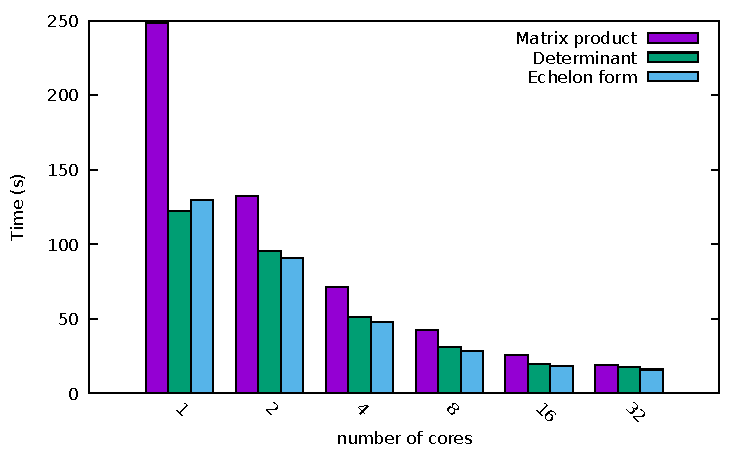
\includegraphics[width=.8\textwidth]{Pictures/histo_bigfoot3}
    \caption{Parallel computation time for some finite field linear algebra operations in SageMath on a 32 core Intel
      Xeon 6130 Gold. Matrices are $20\,000\times 20\,000$ with full rank over $\mathbb{Z}/1\,048\,573\mathbb{Z}$. }
    \label{fig:histo_sage}
  \end{center}
\end{figure}
The speed-up relative to a single threaded run of these timings is reported in Figure~\ref{fig:speedup_sage}
\begin{figure}[htb]
  \begin{center}
    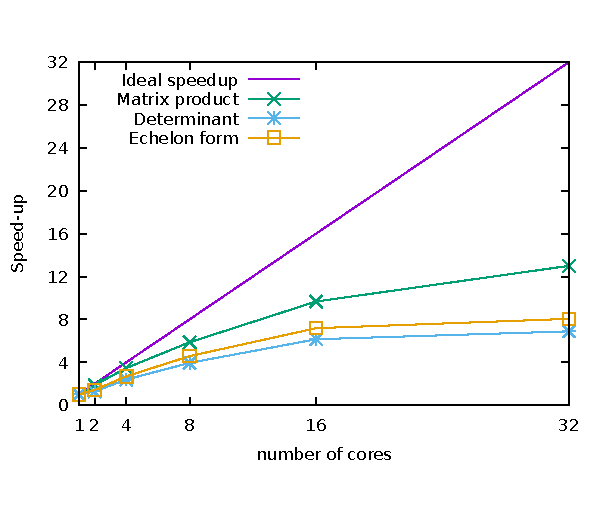
\includegraphics[width=.7\textwidth]{Pictures/speedup_bigfoot3}
    \caption{Parallel speedup for some finite field linear algebra operations in SageMath on a 32 core Intel
      Xeon 6130 Gold. Matrices are $20\,000\times 20\,000$ with full rank over $\mathbb{Z}/1\,048\,573\mathbb{Z}$.}
    \label{fig:speedup_sage}
  \end{center}
\end{figure}

The scalability shown on Figure~\ref{fig:speedup_sage} is good but not close to the best theoretical linear
speedup. This happens for the following reasons:
\begin{itemize}
\item First, the interface between the system \SageMath (running an interactive ipython) and the compiled code of the
  library adds a constant overhead despite our efforts to reduce it as much as possible. According to Amdahl's law~\cite{amdahl67},
  such an overhead severely penalizes the speedup measured;
\item The use of sub-cubic arithmetic for the sequential matrix product tasks implies that the workload increases with
  the number of cores. Therefore, the true ideal speed-up curve should lie slightly below the main diagonal;
\item We did not disable the turbo-boost on this server. Consequently, runs on few cores are likely executed at a higher
  clock frequency, hence penalizing the speedup for large numbers of cores.
\end{itemize}

Still, these timings show that very high performances can be attained directly from the high level interface of
\SageMath, for instance the computation speed on 32 cores reaches 838Gfops\footnote{$1\text{Gfops} = 10^9$ field
  operations per second.} for matrix multiplication and 301 Gfops for
the determinant.

\subsection{Multi-threaded \Singular}

In~\delivref{hpc}{singular-polyarith} we report on parallelisation of
multivariate polynomial arithmetic in \Singular. This is achieved by
outsourcing multivariate polynomial arithmetic to the C \FLINT library
and implementing parallelism there using a data representation
optimised for that purpose (\Singular's primary data representation of
multivariate polynomials is in contrast optimised for Gr\"{o}bner basis
computations, which can themselves be components of a parallel computation
using \Singular's parallel library infrastructure).

As of now, the new parallel multivariate polynomial implementation is available in the
latest development version of \FLINT and \Singular. This will have clear benefits for the
\Singular community and VREs built around \Singular itself, e.g. via the Jupyter front end
for Singular developed as part of \longdelivref{UI}{ipython-kernels-basic}.

The strategy for exposure in \SageMath is that this will be automatic the next time the
version of \Singular is updated in \SageMath. This is possible as the improvements are accessed
through already existing interfaces.

An alternative for the \SageMath project is to wrap the new multivariate interface of \FLINT
directly. However this would be a significant undertaking dependent on the \SageMath
community itself. \FLINT is already a component of \Sage, but at the library level, the new
implementation is a completely new, and quite extensive, interface.

It is expected that the next production version of \Singular will be due in the coming winter
under \Singular's approximate yearly schedule.

The step of updating the version of the \Singular computer algebra system supported in \SageMath
is normally taken care of by the \SageMath community. The effort required is proportional to the
number of changes in the \Singular interface. As a computer algebra system, \Singular is
much more extensive than a narrowly focused library, therefore this effort can still be non-trivial.
It should be noted that this effort is not impacted by the new parallel multivariate implementation
as we have been successful in not changing the \Singular interface to support it. However, all
the other usual work of updating the \Singular version, with its extensive interface that touch
many aspects of \SageMath still needs to be carried out at the next release.

Thanks to independent work, the next production release of \Singular will also include one or
more of the following: fast rational functions, factorisation, additional polynomial orderings
and Gr\"{o}bner basis speedups that directly build on the new parallel multivariate arithmetic.
The work to speed up multivariate arithmetic in \Singular is complete as part of
~\delivref{hpc}{singular-polyarith} and independent work to speed up rational functions is almost
complete. It can thus be expected that \SageMath users will benefit from all these new features at
the time of the next \Singular update in \SageMath.

\Singular also independently provides other mechanisms for parallel code, e.g. via its parallel
library and through the HPC Singular project, which provides parallelism at a coarser grain than
the fine grained parallelism implemented in the new multivariate arithmetic. \SageMath already
has a well-developed interface for accessing \Singular libraries and \SageMath developers can already
benefit from this, due to the fact that anything that works at the \Singular interpreter prompt
also works in \SageMath.

We refer to ~\delivref{hpc}{singular-polyarith} for tables showing the speedups expected at the
\Singular level and a discussion of the differences with a direct interface to \FLINT.

\subsection{Multi-threaded \Pari}

As reported in \delivref{hpc}{pari-hpc2}, the number theory library \Pari supports
multi-threading for various operations.
\Sage uses \Pari for much of its number theory functionality.
As \Sage already interfaces \Pari, a similar situation exists for \Pari-MT (the multi-threading-enabled
configuration of \Pari) in \SageMath as for \Singular. As soon as the next update of the version of
\Pari in \SageMath is completed, parallelism can be enabled in \Pari-MT.

Some experiments have already been conducted in this direction and the \Pari-MT interface can be
made to work in \SageMath with minimal effort under the standard assumption that it is not itself
called from multiple threads not under the control of \Pari.

For example, the documentation builder of \Sage currently uses \Pari to create images for
documentation. However, to handle the hundreds of pages of the documentation -- it uses Python's
multiprocessing module, which (perhaps confusingly) also uses multiple threads.

We expect that this problem can be easily solved with some additional effort in either the \Sage--\Pari
interface or within \Pari itself, for example by enabling run-time configuration of whether to use
sequential or parallel computation in \Pari.

Nevertheless, PARI-MT is usable in SAGE if one is careful not to build the
documentation in this mode, nor to call PARI functions from SAGE-level
threads. It is expected that remaining issues will be resolved in a future \SageMath
release.

We refer again to \delivref{hpc}{pari-hpc2} for details on the expected benefits, which should translate
directly to \SageMath users, due to the straightforward strategy employed: speed up \Pari through threading
without changing the interface.

\subsection{HPC GAP}

HPC \GAP has been in development for very many years, and is now esssentially stabilised in the
main \GAP repository through an extensive recent effort of the \GAP community. It is
even able to be used with a small patch applied to an \emph{existing} \GAP release.

It is not currently possible to use HPC \GAP through the \texttt{libgap} library, however
independent work is currently being undertaken by the main developer of HPC \GAP to make this
possible. This is the preferred way of accessing the \GAP system from \SageMath.

For the purposes of an HPC enabled \Sage distribution, HPC \GAP should perhaps better be viewed as a
standalone application, distinct from \GAP itself. This may even remain the case into the
foreseeable future, as single threaded performance is lower in HPC \GAP than \GAP itself, and compile
time flags are required to enable HPC \GAP, as a result. Further tuning may eventually alleviate some
of this.

There are already some \GAP projects that have taken advantage of HPC \GAP, though the
tool is very new for the \GAP community. It is expected that the \GAP community will develop
many novel uses that benefit from parallelisation. These could be interfaced by the \SageMath
community in the future, at least for very large, specialised projects and parallel computations
that cannot be carried out with the existing serial project.

For further details on \texttt{libgap} and HPC \GAP, see~\delivref{hpc}{GAP-HPC-report}.

%%%%%%%%%%%%%%%%%%%%%%%%%%%%%%%%%%%%%%%%%%%%%%%%%%%%%%%%%%%%%%
\section{Challenges of composing parallel software systems}

As mentioned above, we have been successful in either integrating improved libraries
or interfacing to the external computer algebra systems in most cases without adding to
the maintenance burden of \SageMath.

We now summarise the current situation before discussing what we have learned through
the exchange of expertise about further enhancing \SageMath's HPC capabilities:
\begin{itemize}
\item It is to be expected that \Singular's parallel features will be
  available in the production release of \SageMath by next spring.
\item For the time being it won't be possible to expose HPC-\GAP parallel
  features to \SageMath via its main library-level interface to \GAP. On the
  other hand, they should be accessible to advanced users for hand-launched
  computations, with a separate installation of HPC-\GAP and \Sage's legacy
  text-based interface to \GAP in the near term and via \texttt{libgap} when
  support for HPC \GAP is added by the HPC \GAP developer. It could also be
  possible to use remote procedure calls to an HPC-\GAP 
  server which runs using the SCSCP \GAP package.
\item It is possible right now, with a custom build, to use the development
  release of \Pari compiled to use multithreading, in \SageMath;
  some simple benchmarks demonstrate that \Sage benefits properly from the
  parallel features.
\item Benefits of the the parallel finite field linear algebra library \Linbox
  will be directly enabled in the upcoming release 8.9 of \SageMath which is in
  beta release at the time of writing.
\end{itemize}

We note that all of these features work, or will work, so long as they are in
control of the threads being allocated. However, a full-featured HPC enabled
\SageMath could hope for much more. In particular, we identify a number of levels
of integration that could be expected in the future, each requiring progressively
more effort.

\begin{itemize}
\item HPC components usable from \SageMath independently from a single \Python
  thread. User controls the number of threads.

\item \SageMath controls the number of threads in use by the individual systems,
  but with the same other limitations as the first point.
  
\item The HPC components are able to be run from libraries making use of the
  Python multiprocess model, with tweaks to prevent conflicts, but with much
  reduced performance.
  
\item A fully-fledged HPC Sage distribution with full performance, no limitations
  with regard to multiprocessing and full control over the number of threads
  across the whole system.
\end{itemize}

Obviously the first level of integration is available in the near future as \SageMath
begins to integrate the work completed in the OpenDreamKit project in its normal update
cycle.

As we detail in the next Section, the final level of integration would likely require an unprecedented level of
cooperation, expertise, planning and effort across many projects and across continents.

\subsection{Challenges for producing a fully-fledged HPC \SageMath distribution}

Through the expertise we have gained across OpenDreamKit and by consulting outside
experts, we have compiled a list of the challenges to producing a fully-fledged
HPC Sage distribution. These are in fact challenges to any sufficiently large system
and especially apply to Open Source distributions which combine disparate projects
developed across a wide range of communities.

In the points we identify, we refer to both process level parallelism and thread level
parallelism. Both come with advantages and disadvantages. But the most important point
in either case is that the components of the system need to agree on a common strategy
for parallelism, including a strategy for how the two kinds of parallelism should
cooperate. This is the overarching obstacle to producing an HPC Sage, because the individual
components have not been designed, a priori, with such cooperation in mind from the ground up.

By ``strategy'' here, we mean how one should write parallel code across the whole system, how
threads and processes should coordinate and how memory should be cooperatively managed.

Threading components cooperatively present many technical challenges, especially in a
heterogeneous system. In particular, components need to agree on how to make code threadsafe,
how to control the number of threads and how to share memory when threads are started in the
same process, and then this strategy needs to be rolled out across all components. Libraries
that are currently not threadsafe then need to be made threadsafe, which can mean extensive
reworking or use of automated tools such as those used in the parallel \Singular system.

A multiprocess approach may avoid some of the technical obstacles presented by threads, but
then one needs to decide how to do data sharing and communication between processes.

We present a (non-exhaustive) list of some of the specific technical obstables that must be
overcome to create a working, fully-fledged HPC distribution:

\begin{itemize}
\item Garbage collectors: these need to be thread aware and to cooperate with one another.
  Typically they aren't and they don't. It's not sufficient for each system to have threaded
  garbage collection (gc), as allocations in one system can trigger allocations in another, e.g.
  with recursive structures from one system built on structures from another system. If the
  gc of one system is not aware of the threads of the other system, this will lead to crashes.

\item Data sharing: e.g. a GMP integer created in one system can't be handed to another system
  and freed or even used there because bit level gc flags prepended to the data will be different
  and different allocators work in different ways. This means data typically has to be copied
  everywhere even at a very low level, causing very high overhead when transferring information
  from one system to another.

\item Initialisation: some packages and libraries need special per thread initialisation. For
  example, HPC \GAP requires per thread initialisation of interpreter state. This works well in a
  system where \GAP is controlling the whole system, but if another part of the system needs to
  start up threads, it has to hook into the library initialisation of HPC \GAP. This is difficult,
  technical work and will only interoperate with other systems that have been specifically
  designed to cooperate with it.

  This problem is particularly acute when using packages as libraries, e.g. via \texttt{libgap}.

\item Threaded allocators: although the system malloc is threadsafe, it is not efficient in a
  multithreaded environment, especially on OSX. Allocators such as Singular's omalloc are not
  threadsafe at all and there is a uniform slowdown of 2x using the system allocator, across
  the whole system. High performance threaded allocators such as tcmalloc don't alleviate this
  problem, and in the worst case make it even worse. This is because custom allocators are
  heavily tuned for the systems using them. Writing parallel custom allocators is extremely
  demanding work, which can take years of effort. Without them, large slowdowns may occur when
  running an HPC aware system in a single core environment.

\item Thread safety: many libraries are not threadsafe, and making them threadsafe can be a major
  undertaking, for example eliminating global variables, or putting mutexes on them, linking against
  threadsafe allocators, having functions not modify their inputs, etc. Many libraries are currently
  written without these requirements in place, meaning they would have to be rewritten from scratch
  on any system that makes calls out to them from another threaded library. Otherwise, parts of the
  system would have to be turned off in a threaded environment.

  This is not just a theoretical problem. Singular for example can make use of coefficient rings
  provided by other systems. Parallel Gr\"{o}bner basis code may then result in the provider of those
  coefficient rings needing to be made threadsafe. Other packages maintain global characteristics, e.g.
  a modulus, which may be set and reset by different threads calling that code, resulting in inconsistent
  and incorrect results, which may not be detected until the code is run for the first time, or at all.
  In the worst case, this can result in publications having to be withdrawn because computations appeared
  to output meaningful results, but in fact were corrupted at run time.

\item Thread control: it is very expensive on a supercomputer where time has to be paid for by core/hour if
  thousands of threads are started by the system because there is no uniform control to limit the number of
  threads. Failure to implement such a mechanism could cost users tens of thousands of dollars. We are aware
  of an instance where this happened to a colleague because they decided to roll their own parallel code.

\item Compiler/interpreter cooperation: threaded gc usually requires cooperation and integration with the
  language(s) themselves. Retrofitting this kind of functionality to a language not designed to work with
  threaded gc is usually impossible, as languages tend to be developed by external communities and are not
  under the control of package developers. The work is also extremely technical and complicated.

\item Different gc strategies: compacting, moving, incremental, precise, conservative, reference counting,
  generational. All the different collectors have different strategies, which make different assumptions,
  especially about object references from the stack or in CPU registers, and different assumptions about
  reachability, when collection can happen and what mechanisms exist to make this threadsafe. If a system
  requires threads to be stopped in order for part of its gc cycle (typical) then other threads can't just
  keep going and potentially triggering allocations during that time. Simply stopping everything for all
  the different allocators may lead to very poor performance across the system.

  References from one gc memory space to another need to be managed, typically with finalizers, which can
  be a performance bottleneck, and cycles overlapping different gc memory spaces cannot be effectively handled,
  placing limitations on the types of structures that can be constructed by the system, which may place
  additional constraints on the mathematical user.

\item Memory monitoring: many allocators more agressively clean up memory when it is running low. But in
  order to do this, they need reliable information about how much has been allocated. This is typically done
  by counting allocations across the system. But each collector needs this information and it needs to be
  shared across all the systems. 

\item Bugs: there's a saying that at scale, everything breaks. Whilst single core systems are often very
  tolerant of coding bugs, parallel code will expose a great number of bugs that were previously hidden. A
  small memory leak here, or an array overrun there will cause massive corruption or out of memory conditions
  or crashes in a parallel system.

\item Tools: debugging multithreaded applications usually requires integrated tools that are aware of all
  parts of the system. It is not feasible to write and debug code that cannot effectively be debugged. It
  just causes massive delays in development of new features across the system, effectively bringing
  development to a halt. It is typical for a single bug in a multithreaded or multiprocess system to take
  months to resolve without such tools. Profilers similarly need to be thread/process aware and may need
  integration with the system to monitor it effectively.

\item Language features: use of a parallel system usually requires new language elements, e.g. semaphores,
  mutexes, shared regions, coroutines, tasks, etc. Development of these can be prohibitive in systems designed
  around languages which do not have these features. For example, tasks in Gap need to cooperate with tasks in
  Python, otherwise neither will function.

\item Heterogeneous computing: very often the resources that are available differ from site to site, or may
  even be heterogeneous at a given site. E.g. the code may be running on a local server, but computing
  resources may exist over a network on a large supercomputer. This is expected to be increasingly the case in
  future years as Moore's law for desktop computing comes to an end. Effective use of external resources
  requires significant understanding of the technologies that enable this, and integration of those
  technologies into the system, often with language support being required.

\item Platform and architecture support: often, getting high performance in parallel workloads depends on
  being able to natively support the operating system or architecture. Large packages like \GAP and \Singular
  do not have native Windows versions. Moreover, tricks such as thread local storage can be inefficient on
  certain operating systems, meaning that significant rework of package code at a very technical level may
  be necessary to retrofit them for efficient parallel operation.
\end{itemize}

All of these obstacles show that whilst our efforts toward an HPC \Sage distribution are vital, they are
just the beginning of what will be a long journey!

\bibliographystyle{acm}
\bibliography{D3.11}
\end{document}

%%% Local Variables:
%%% mode: latex
%%% TeX-master: t
%%% End:

